\begin{figure}[t]
	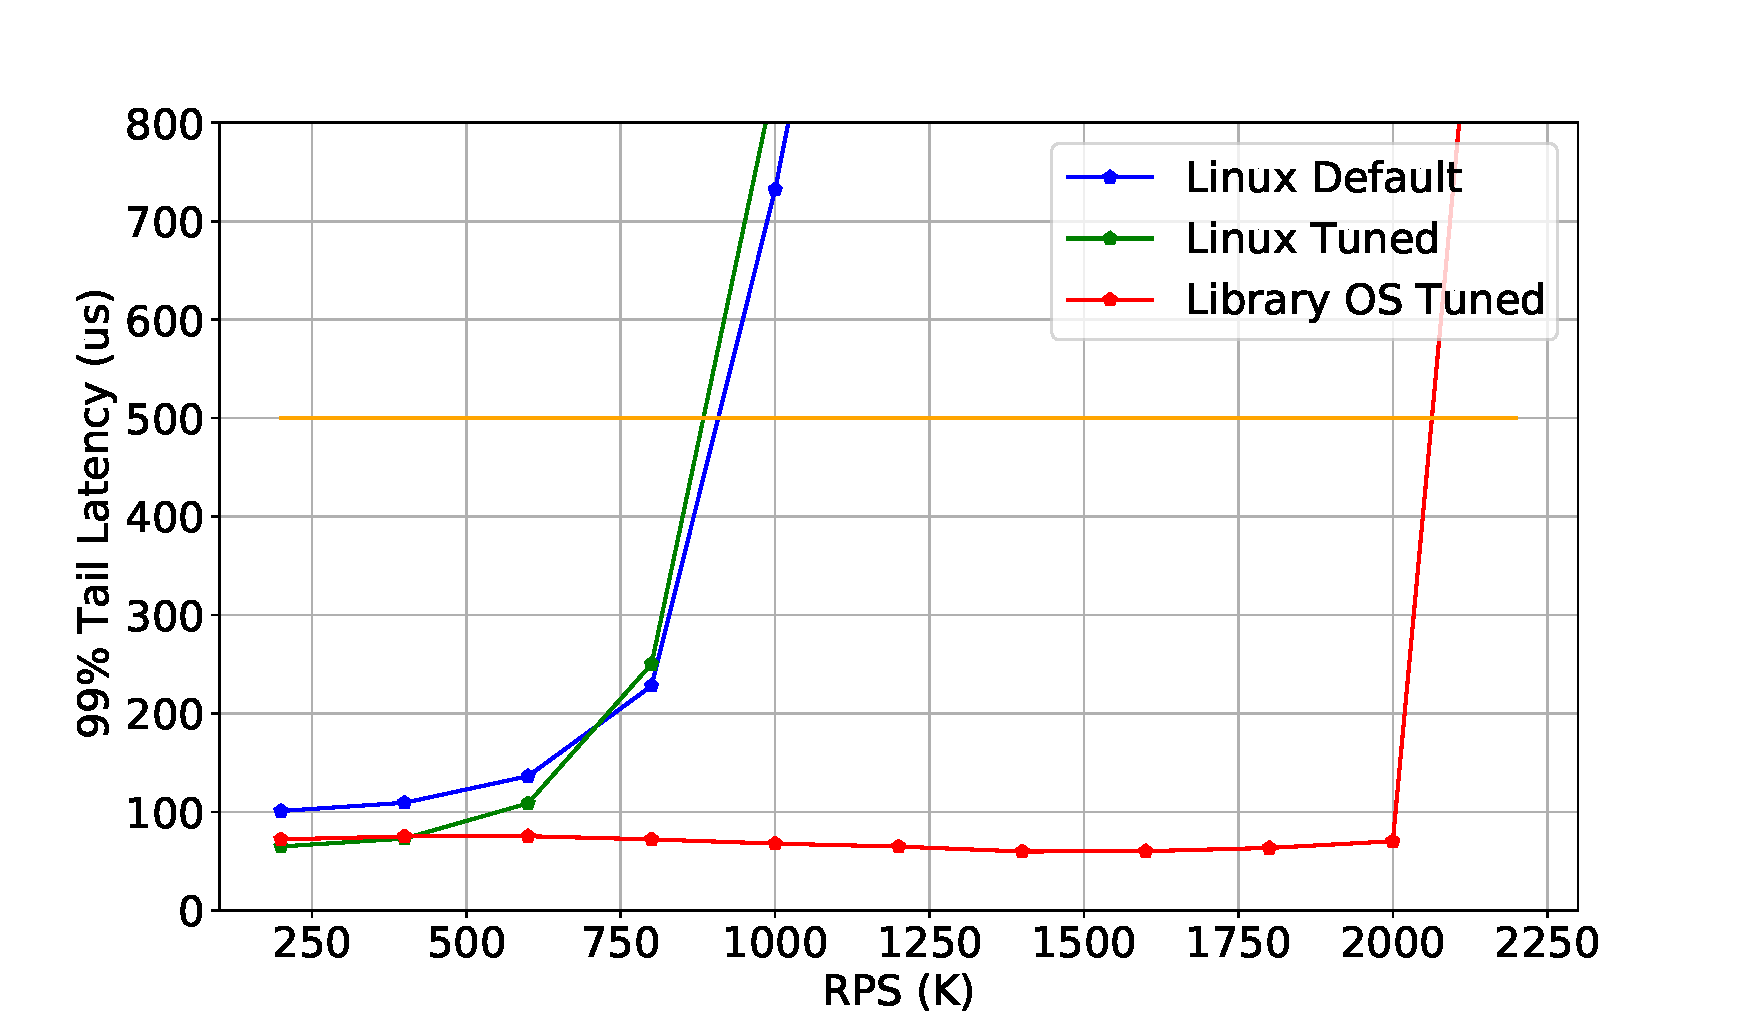
\includegraphics[width=\columnwidth]{asplos2021_figures/mcd_sla.pdf}
	\caption{Performance measure of memcached such that 99\% tail latency < 500 $\micro$s SLA.}
	\label{fig:mcd_sla_tot}
\end{figure}

Figure~\ref{fig:mcd_sla_tot} compares the base performance between Linux default and the two systems when tuned for performance. Given that this is a complicated multicore workload with mixed request rates and the need to satisfy a stringent SLA; tuning hardware parameters in Linux does not produce a noticeable increase in overall peak throughput (but does achieve lower tail latency at low QPS rates). This result is not surprising given the enormous efforts from past researchers to understand and optimize the network paths for workloads such as memcached~\cite{tailatscale, scalingmcdfacebook, workloadanalysisfacebook, ix, ebbrt, farm, 222583}.  The libOS systems optimizations coupled with its baremetal network device driver both contributed to its 2X throughput improvement over Linux.

\subsubsection{General Observations}
Table~\ref{table:eppsum} shows that tuning Linux can lower its EPP by up to 22\% while tuning the libOS can lower its EPP by up to 74\%. For the libOS, we find in all the different cases of QPS loads, that the best ITR value was 2 \micro s; which is the lowest value possible. For tuned Linux, the best ITR values range from 10 \micro s at the lowest offered load up to 30 \micro s at the highest QPS load studied. At low QPS stuned Linux hovered around the midrange for both DVFS (\texttt{0x1500}) and RAPL (\texttt{75}) and at the highest QPS load of 600K, tuning Linux found its minimum EPP with DVFS and RAPL at the highest setting while libOS was able to set ITR, DVFS and RAPL all relatively low. This result is not surprsing given the throughput performances in figure~\ref{fig:mcd_sla_tot} as a QPS of 600K is considered relatively light for the libOS while for Linux it is approaching its peak. Examining the log data we also found that across all the QPS loads, the minimum EPP value for tuned Linux always resulted in increase of its energy use (7.5\%) over Linux default while having a lower 99\% tail latency (22\%). Whereas libOS' minimum EPP consisted of both reductions in 99\% tail latency and energy by up to 56\% and 40\% respectively.

\subsubsection{High ITR Delays}
Another interesting tradeoff can be observed in overview figure~\ref{fig:mcdov}, where tuned Linux can drastically lower its energy consumption by up to 50\% if it is willing to sacrifice most of its 500 \micro s SLA budget. We find this is possible by aggressively setting ITR delay at much higher values of 300-400 \micro s. Using an offered load of 600K QPS as an example, we find that compared to default Linux, a tuned Linux with an ITR delay of 300 \micro s can lower its energy use by 44\% through a combination of: 1) 93\% reduction in total interrupts, 2) 30\% reduction in instruction use and last-level cache misses, and 3) a 12X increase in C1E, C3 sleep states, and 2X increase in C7 sleep states. To summarize, tuning Linux with a high ITR delay allows it to go to deeper sleep states and more often, further, the amount of reduced interrupt contents also contributed to less code being executed overall. Moreover, we find that it is able to lower its DVFS at a lower level than tuned Linux for minimum EPP, we hypothesize this is related to the fewer amount of non-application related work that is being done. We do not observe this dramatic of an energy savings in the libOS (only 14\% at 600K QPS), we suspect this effect comes into play at greater efficiences only at much higher QPS for the libOS. There have been a plethora of past work in reducing energy use of workloads such as memcached as it exhibits a diurnal pattern where periods of low utilization exist~\cite{workloadanalysisfacebook, 10.1145/2024723.2000103,10.1145/2678373.2665718, 10.1145/2806777.2806848}, tuning ITR delay can be an additional lever to further reduce a systems' overall energy use. 

\begin{figure}[t]
	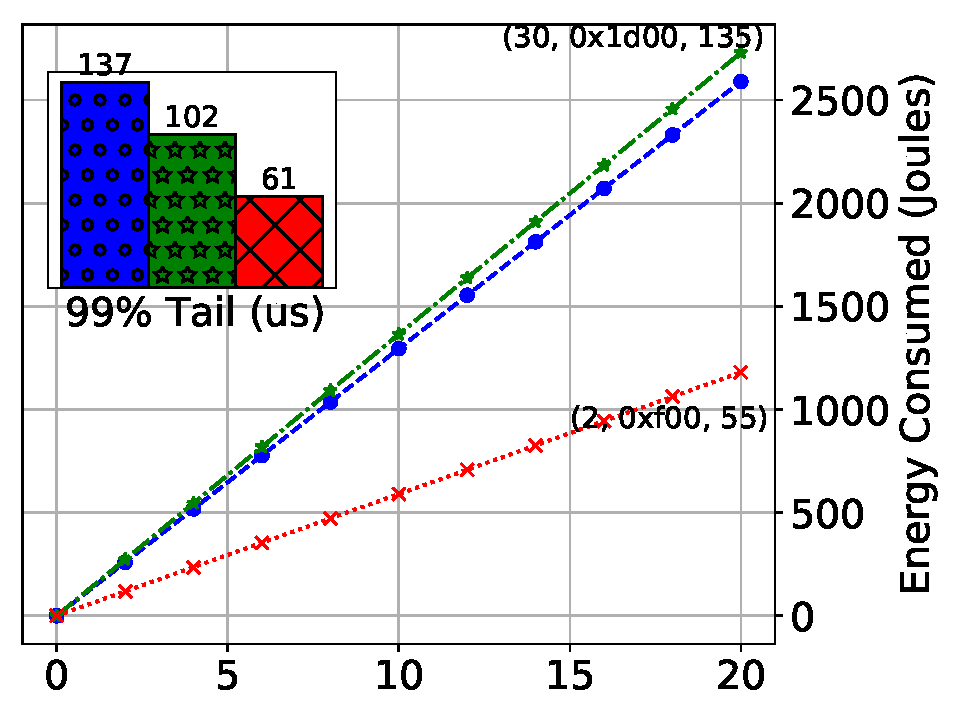
\includegraphics[width=\columnwidth]{osdi_figures/mcd_600000_epp.pdf}
	\caption{Memcached EPP plot across three systems at 600K QPS.}
	\label{fig:mcd_600000_epp}
\end{figure}
\begin{figure}[t]
	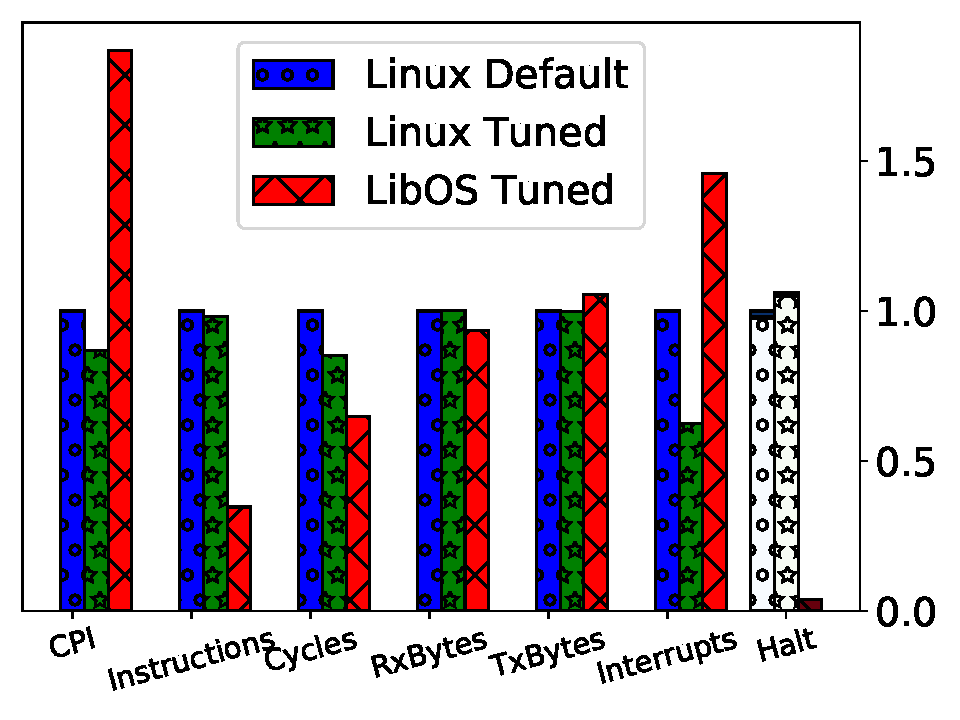
\includegraphics[width=\columnwidth]{osdi_figures/mcd_600000_barplot.pdf}
	\caption{Collected datapoints of memcached across three systems normalized to Linux Default.}
	\label{fig:mcd_600000_bar}
\end{figure}
\begin{figure}[t]
	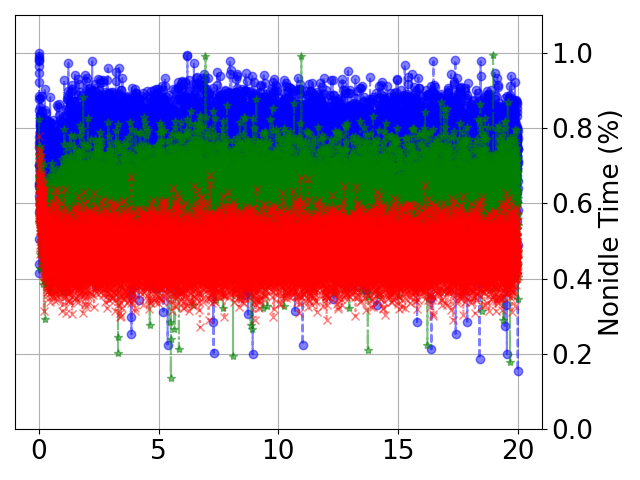
\includegraphics[width=\columnwidth]{osdi_figures/mcd_600000_nonidle_timeline.png}
	\caption{Memcached 600K QPS per-interrupt non-idle ratio.}
	\label{fig:mcd_600000_nonidle}
\end{figure}

\begin{figure}[t]
	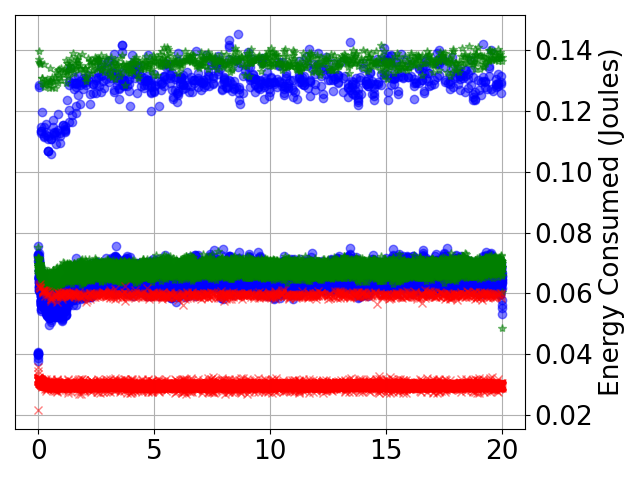
\includegraphics[width=\columnwidth]{osdi_figures/mcd_600000_joules_timeline.png}
	\caption{Memcached 600K QPS per-interrupt joule consumption.}
	\label{fig:mcd_600000_joule}
\end{figure}


\subsubsection{600K QPS Analysis}
Figure~\ref{fig:mcd_600000_epp} shows the energy as a function of time across the three systems with minimum EPP. We highlight the 99\% tail latency differences between the three systems as well. In this example, tuned Linux used 5\% higher energy than Linux default while reducing its tail latency by 26\%, libOS used 56 \% less energy and reduced its tail latency by 40\%. Given that memcached is a less compute intensive workload, it is not a surprise that reducing tail latency is important for both tuned Linux and libOS. However, what is surprising is the different combination of ITR, DVFS, and RAPL setting that each system took. The libOS used the lowest ITR value possible (2 \micro s) and set its DVFS/RAPL at the middle ranges, this helped to contribute to its 50\% increase in number of interrupts compared to Linux default. The general efficiency and smaller size of the libOS can be seen in figure~\ref{fig:mcd_600000_bar} as even with the extra interrupt counts, the libOS' instruction count was 65\% less than Linux. This efficiency enables libOS to minimize its 99\% tail latency while using less energy. Even though figure~\ref{fig:mcd_600000_bar} shows that the libOS went to \texttt{C7} sleep state over 2X more than Linux default, we do not believe it actually stayed in those a \texttt{C7} sleep state given its exit latency (hundreds of \micro s) and the dynamic nature of the workload with such a low ITR delay that will constantly waking up the processor. The biggest indication of tuned Linux's difference from default Linux is in the interrupt count, which is 30\% less than Linux default, we attribute this to its ITR delay value of 30 \micro s. This ITR delay seems to shift the ratio of sleep states to focus on \texttt{C1} and \texttt{C1E}, overall it seems tuning Linux allows it to \texttt{halt} more often than Linux default. Figure~\ref{mcd_600000_nonidle} also supports this why showing that tuning Linux spent less time being busy than default. Tuned linux has lower CPI than default, an indication of why it managed to achieve lower tail latency. While tuned Linux was able to be scheduled to sleep more often, it consumed energy at a higher rate than default, could be the exit latencies of more sleep states given the dynamic nature of memcached workload.


%This result demonstrates a distinct tradeoff being made by Linux in terms of how it reached the minimum EPP possible. 
%In contrast to the NAPI polling policy, EbbRT is not limited by a polling budget per receive interrupt, it will process as many receive descriptors as the hardware allows in a synchronous manner, moreover as interrupts are disabled during this entire process, EbbRT potentially could process more packets than Linux which must balance workload with processing budgets.
%Given the base performance of each system, f
%Figure~\ref{fig:mcd600K} illustrates the base energy costs when tuning Linux and library OS to minimize EDP. Similar to nodejs, we also scale the log data to show a fixed workload of 5 million requests for each system and the results we present below is for the 600K QPS rate. We noticed there was a discrepancy in the raw data logs only for Linux tuned in reported EDP values, therefore in figure~\ref{fig:mcd600K} we show the EDP for each run of all systems. It is something we are currently investigating.  However, the results we present regardless show significant differences in the system beyond the displayed variance.  

%While Memcached and the mutilate workload are more represented of a real world cloud service component and load.  It raises interesting challenges from an EDP analysis perspective.  Given that the benchmark generates the requests from a distribution over the request times (gets and sets of particular keys and data) there is no real fixed work rather it is a sample of work.  To this end we plot EDP curves from multiple runs given the observed variance.  While there is variance the optimized EDP shows distinct separation between the systems greater than the variance.  

% fixed tuning what kind of benefit over base Linux,
% what influence does having shorter code paths on tuning, 
% what does getting to sleep/idleness difference, 
% are you exploiting to sleep, synergistic with instruction efficiency,

%% \begin{figure}
%% 	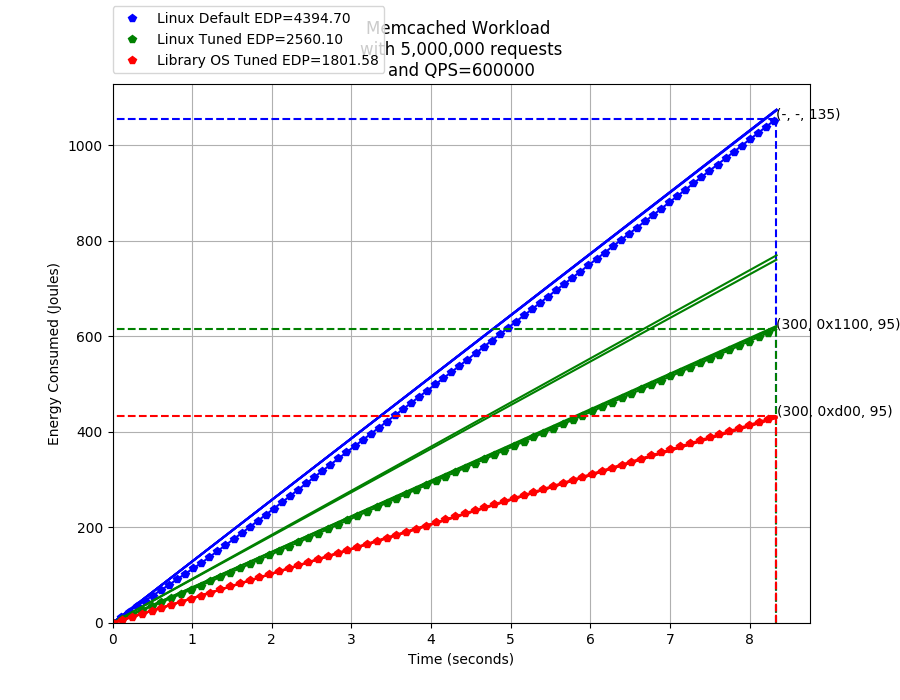
\includegraphics[width=\columnwidth]{asplos2021_figures/mcd_edp_QPS600000.png}
%% 	\caption{Minimum EDP plots when tuned for lowest energy use.}
%% 	\label{fig:mcd600K}
%% \end{figure}

%% \begin{figure}
%% 	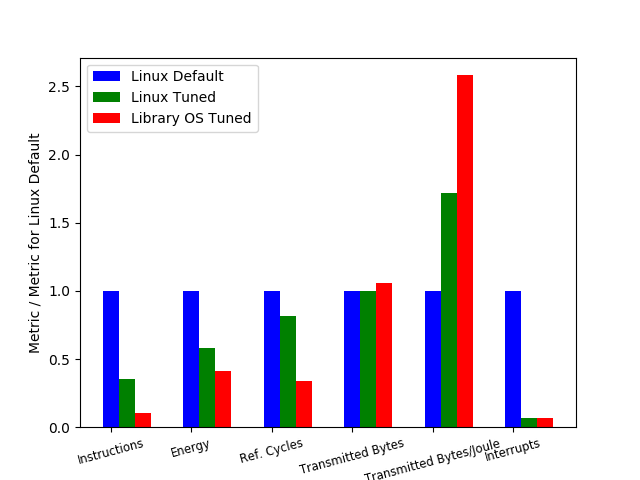
\includegraphics[width=\columnwidth]{asplos2021_figures/mcd_combined_barplot_QPS600000.png}
%% 	\caption{Summed up measures from logs and normalized against Linux default.}
%% 	\label{fig:mcdbar600K}
%% \end{figure}

%As stated in the introduction there are dramatic energy saving when comparing the default Linux behavior to statically setting the hardware parameters as is evident in Figure~\ref{fig:mcd600K}.  Perhaps what is most surprising the trade-offs and causality observed in the simpler benchmarks result in a significant win under a far more complex load.  By-passing Linux default behaviour yields similar wins with respect to reducing the utilization between interrupts as indicated in Figure~\ref{fig:mcdnonidle600K}. Specifically, we find the improvement in interrupt processing leads respectively to decreases in nonidle times for both Linux and the Library OS and that these directly are exploited by the idle polocies to dramatically reduce energy.  

%Perhaps one of the most interesting observations comes from the modest QPS of 600k that we have chosen to highlight.   While there are interesting phenomena at higher QPS that the Library OS can support and Linux cannot it is important to note that Tuning has dramatic impacts even in under-loaded senearios.  While attention is usually given to analyzing memcached's performance at high load there is critical headroom for significantly improving the efficiency when servers are operating at lower loads.    

%In the appendix we have include results from our study of Silo-Memcached which integrates an in memory data-base.  This workload induces a more subtle and complex tradeoff between CPU load and IO latency.  Discussion is beyond our space constraints.  
%Although not illustrated we o sweep data reveals that 
%As stated in the introduction 
%The library OS is able to save over 60\% Joules over Linux default by also taking advantage of aggressive interrupt-delay tuning. The drastic difference between the instruction count of the library OS while transmitting slight higher bytes than Linux speaks to the packet processing efficiency. The benefit of a library OS's packet processing efficiency is evident in figure~\ref{fig:mcdnonidle600K} where its non-idle time is roughly half of Linux, another indicator of the ability of a library OS to take advantage of deep sleep states. 




%Our strategy for tuning interrupt-delay is also influenced by previous observations from past work on studying memcached workloads where it can operate in low to medium utilization levels due to diurnal patterns in user traffic~\cite{workloadanalysisfacebook, 10.1145/2024723.2000103}. One way to save energy is to scale a node's energy consumption down under low to medium utilization while satisfying the current SLA. Prior research have tackled this specific problem by using DVFS and RAPL~\cite{10.1145/2678373.2665718, 10.1145/2806777.2806848}. In our study, we take a much wider range of interrupt-delay values (up to 400 $\micro$s) and found that by add aggressive delays in packet processing interrupts, it allows to drastically lower the amount of interrupts to handle and enable better packet processing (shown figure~\ref{fig:mcdbar600K}). By combining this with lower DVFS and RAPL values, it enabled Linux tuned to save between 20\% and 40\% Joules over default. 





%% \begin{figure}
%% 	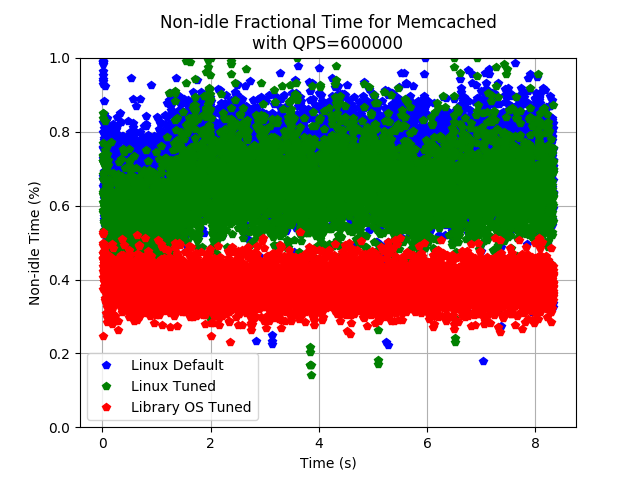
\includegraphics[width=\columnwidth]{asplos2021_figures/mcd_nonidle_QPS600000.png}
%% 	\caption{Per interrupt measure of non-idle time computed using fixed reference cycles.}
%% 	\label{fig:mcdnonidle600K}
%% \end{figure}

